%FOR PDFLATEX USE ONLY
\documentclass[a4paper,12pt]{article}

\usepackage{amssymb,amsmath}

\usepackage[margin=2cm]{geometry}
\usepackage[unicode]{hyperref}
\usepackage[pdftex]{graphicx}
\usepackage{cmlgc}

\usepackage{array}

\usepackage{wrapfig}
\usepackage{array}
\usepackage{lipsum}
\usepackage{esvect}
\usepackage{hyperref}

\usepackage{subfig}
\usepackage{calc}
\usepackage{pgfplots,tikz,circuitikz}
\usepackage{pgfplotstable}
\usepackage{tkz-euclide}

\usepackage{centernot}
\usepackage{cancel}

\usepackage{mathtext}
\usepackage[T1,T2a]{fontenc}
\usepackage[utf8]{inputenc}
\usepackage[english, bulgarian, russian]{babel}
\usepackage{tikz}
\usepackage{pgfplots}
\usepackage[export]{adjustbox}
\usepackage[left=2cm,right=2cm,
    top=2cm,bottom=2cm,bindingoffset=0cm]{geometry}
\usepackage{indentfirst}
\usepackage{braket}
\usepackage{booktabs}
\usepackage{multirow}

\begin{document}

\begin{center}
  \LARGE{Работа 2.1.3}\\[0.2cm]
  \LARGE{Определение $C_p/C_v$ по скорости звука в газе}\\[0.2cm]
  \large{Малиновский Владимир}\\[0.2cm]
  \normalsize{\texttt{galqiwi@galqiwi.ru}}
\end{center}

\textbf{Цель работы:} Измерение частоты колебаний и длины волны при резонансе звуковых колебаний в газе, заполняющем трубу

\textbf{В работе используются:} звуковой генератор ГЗ, электронный осциллограф ЭО, микрофон, телефон, раздвижная труба, теплоизолированная труба, обогреваемая водой из термостата, баллон со сжатым углекислым газом, газгольдер.

\section*{Описание работы}
Из теории нам известна зависимость скорости звука от показателя адиабаты $\gamma$:
$$c = \sqrt{\gamma\frac{RT}{\mu}}.$$
Таким образом, задача нахождения $\gamma$ сходится к задаче нахождения скорости звука при заданной температуре.\\
В этом эксперименте предпологается использовать стоячие волны для нахождения $c$. Известно, что стоячие волны в коридоре длиной $L$ образуются при:
$$L = \frac{n}{2}\lambda,$$
где $\lambda$ -- длина волны звука, связанная со скоростью звука и частотой $f$, как:
$$\lambda = c/f.$$
То есть верно, что:
$$L = \frac{c}{2f}n.$$
В текущем эксперименте мы будем знать не абсолютный номер порядка $n$, а его приращение $k = n - n_0$, для которого верно, что:
$$\Delta L = L - L_0 = \frac{c}{2f}k + \Delta L_0,$$
где $L_0$ -- минимальный размер трубы, а $\Delta L$ -- отклонение от него, которое мы можем измерить.

\newpage
\section*{Экспериментальная установка}
В этой работе мы будем измерять зависимость $\Delta L(k)$ при постоянных значениях $f$, из чего получим $c$. Для этого мы используем установку на Рис. 1. Эта установка представляет из себя две вложенных друг в друга трубы с миллиметровой шкалой на подвижной части. На краях этой системы установлены приемник Т и передатчик М. Также к системе подведена трубка, через которую можно накачивать пространство внутри труб воздухом или углекислым газом.
\begin{center}
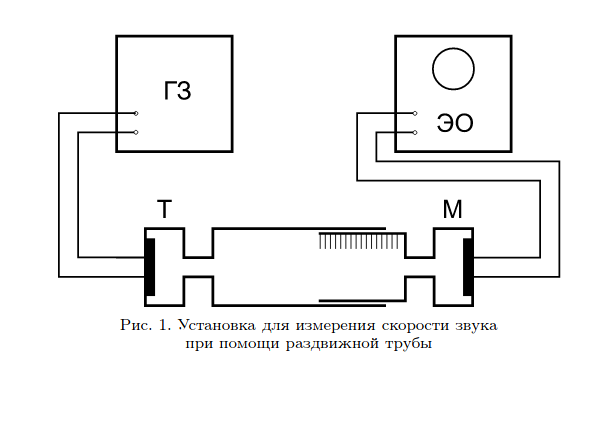
\includegraphics[width=0.95\textwidth]{equip.png}.
\end{center}
\section*{Описание работы и ее результатов}
(1) Включим звуковой генератор с осциллографом и дадим им прогреться 5-7 минут.\\
(2) Зададим амплитуду и частоту сигнала на генераторе так, чтобы на осциллографе можно было пронаблюдать сигнал. Он должен быть неискаженным синусоидальным. Если он будет искаженным, уменьшим амплитуду.\\
(3, а, б, в) При вариации длины в $230 \text{мм}$, для того, чтобы при скорости в $340\text{м}/\text{с}$ было $\approx 4$ резонанса, нужна частота порядка:
$$f \approx \frac{4\cdot340\text{м}/\text{с}}{2 \cdot 0.23 \text{м}} \approx 3\text{кГц}.$$\\
Продуем трубу воздухом $\approx 5 \text{мин}$.\\
Для нескольких частот получим различные зависимости $\Delta L(k)$, плавно вытягивая и втягивая внутреннюю трубку относительно внешней и наблюдая за амплитудой показаний осциллографа. При достижении максимума амплитуды, наблюдается резонанс, и мы записываем новое значение $\Delta L$.

\begin{center}
\begin{tabular}{|c|c|m{0.8cm}|m{0.8cm}|m{0.8cm}|m{0.8cm}|m{0.8cm}|c|m{0.7cm}|m{0.6cm}|m{0.6cm}|c|}
\hline $N_\text{изм}$&$f, \text{кГц}$&$L(0),$ мм&$L(1),$ $\text{мм}$&$L(2),$ $\text{мм}$&$L(3),$ $\text{мм}$&$L(4),$ $\text{мм}$&$\lambda, \text{мм}$&$\Delta \lambda,$ $\text{мм}$&$c,$ $\text{м}/\text{с}$&$\Delta c,$ $\text{м}/\text{с}$&примечание\\ \hline
1&4.00&38&82&126&170&215&88.4&0.2&354&2&вверх\\ \hline
2&3.99&42&85&127&170&215&86.2&0.5&344&3&вниз\\ \hline
3&2.45&12&85&155&223&-&140.6&1.1&344&4&вверх\\ \hline
4&2.45&12&77&120&218&-&132.2&10.7&324&27&вниз\\ \hline
5&1.74&13&112&210&-&-&197.0&0.3&343&3&вверх\\ \hline
6&1.74&10&110&210&-&-&200.0&0.1&348&2&вниз\\ \hline
7&3.25&46&99&152&207&-&107.2&0.5&348&3&вверх\\ \hline
8&3.25&46&100&153&207&-&107.2&0.2&348&2&вниз\\ \hline
9&1.99&9&94&180&-&-&171.0&0.3&340&2&вверх\\ \hline
10&1.99&4&85&178&-&-&174.0&4.0&346&10&вниз\\ \hline
11&2.73&65&130&191&-&-&126.0&1.3&344&5&вверх\\ \hline
12&2.73&64&128&191&-&-&127.0&0.3&347&2&вниз\\ \hline
13&3.75&40&85&132&178&224&92.2&0.2&346&2&вверх\\ \hline
14&3.75&40&84&133&178&225&92.8&0.6&348&3&вниз\\ \hline
\end{tabular}
\end{center}
$$\Delta f = 0.01\text{кГц},\,\Delta L = 0.5\text{мм}.$$
Значение $\lambda$ и ее погрешности я получил через МНК, по формуле
$$\lambda = 2 \frac{dL}{dk}.$$
Приборная погрешность у этого эксперимента сопоставима с погрешностью мнк:
$$\varepsilon f \approx \frac{1}{200} = 0.5\%,$$
$$\varepsilon L \approx \frac{0.5}{100} = 0.5\%,$$
что добавит дополнительные $1\%$ погрешности к финальному результату.\\
Из таблицы видны выбросы на 4 и 10 измерении -- видимо, на них слишком неточно были получены несколько точек. В последующих вычислениях я их не буду учитывать.
Из МНК получается средняя скорость звука:
$$c = (346\pm3)\frac{\text{м}}{\text{с}}.$$
C Учетом $1\%$:
$$c = (346\pm5)\frac{\text{м}}{\text{с}}.$$
Как было сказано ранее, из $c$ мы можем найти $\gamma$ (при $T = (25\pm 5)^\circ C$):
$$\gamma = \frac{\mu c^2}{RT} = 1.40 \pm 0.07,$$
что сходится с теорией.\\
(3, г) Измерение скорости звука в углекислом газе.\\
Измерение скорости звука в углекислом газе проводится аналогично скорости звука в воздухе, но со своими особенностями: установка не является герметичной, и поэтому в нее поступает воздух при движении трубы наружу. Поэтому метод нахождения получает новые особенности:
\begin{enumerate}
	\item Просто открытия краника для того, чтобы закачать $CO_2$, недостаточно -- надо открыть краник и начать вводить-выводить внутреннюю трубу где-то 20 секунд, прокачивая $CO_2$ внутрь, и удаляя воздух.
	\item $CO_2$ надо обновлять после каждого измерения -- это правило я не выполнил в двух измерениях, что указал в таблице, поскольку официальная методика решения была без этого правила.
	\item Измерения проводятся только при входе трубы внутрь. Поскольку измерения при полностью открытом кране невозможны из-за сильного шума на осциллографе, при выводе трубы, в установку закачивается воздух.
	\item Во время измерений краник немного приоткрыт -- достаточно, чтобы был доступ к $CO_2$, но недостаточно, чтобы были помехи в работе осциллографа.
\end{enumerate}


\begin{center}
\begin{tabular}{|c|c|m{0.8cm}|m{0.8cm}|m{0.8cm}|m{0.8cm}|m{0.8cm}|m{0.8cm}|c|m{0.7cm}|m{0.6cm}|m{0.6cm}|c|}
\hline $N_\text{изм}$&$f, \text{кГц}$&$L(0),$ мм&$L(1),$ $\text{мм}$&$L(2),$ $\text{мм}$&$L(3),$ $\text{мм}$&$L(4),$ $\text{мм}$&$L(5),$ $\text{мм}$&$\lambda, \text{мм}$&$\Delta \lambda,$ $\text{мм}$&$c,$ $\text{м}/\text{с}$&$\Delta c,$ $\text{м}/\text{с}$&примечание\\\hline
1&3.25&8&48&89&132&172&212&82.0&0.4&266&2&\\ \hline
2&3.02&12&64&118&174&-&-&108.0&0.9&327&4&без п.2\\ \hline
3&2.74&35&90&149&207&-&-&115.0&0.8&315&3&без п.2\\ \hline
4&2.74&40&88&138&185&-&-&97.0&0.5&266&2&\\ \hline
5&2.23&32&92&153&212&-&-&120.2&0.4&268&2&\\ \hline
6&1.75&78&155&-&-&-&-&154.0&0.1&270&2&\\ \hline
7&1.50&8&105&188&-&-&-&180.0&4.7&271&9&\\ \hline
8&1.99&45&115&177&-&-&-&132.0&2.7&263&7&\\ \hline
9&2.50&55&105&160&213&-&-&105.8&1.0&264&3&\\ \hline
\end{tabular}
$$\Delta f = 0.01\text{кГц},\,\Delta L = 0.5\text{мм}.$$
\end{center}
Как видно из таблицы, значения измерений 2 и 3 выбиваются на фоне других -- видно, что из-за проникновения воздуха, скорость звука вырастает со значений $\approx 265 \text{м}/\text{с}$ до $320\text{м}/\text{с}$, что ближе к $345\text{м}/\text{с}$ воздуха.\\
Аналогично воздуху, найдем $c$:
$$c = (267\pm4)\text{м}/\text{с}.$$
Приборная погрешность так же равна $1\%$. С ее учетом:
$$c = (267\pm5)\text{м}/\text{с}.$$
Из этого $\gamma$ равна:
$$\gamma = \frac{\mu c^2}{RT} = (1.27\pm0.07),$$
что соответствует табличному значению.

\section*{Вывод}
Мы научились измерять показатель адиабаты через скорость звука с помощью резонансных пиков зависимости амплитуды принимаемого сигнала при прохождении в закрытом пространстве от расстояния, проходимого звуком в одну сторону из-за появления стоячих волн, результаты эксперимента совпали с табличными значениями. Был уточнен метод получения скорости звука в углекислом газе.
\end{document}








\lipsum[1-4]
\begin{wrapfigure}{R}{5cm}
\centering
\includegraphics[width=0.20\textwidth]{rd.png}
\caption{1}
\end{wrapfigure}
\lipsum[1-6]


\begin{figure}[h]
\begin{center}$
\begin{array}{cccc}
\includegraphics[width=0.20\textwidth]{rd.png}&
\includegraphics[width=0.20\textwidth]{rd.png}&
\includegraphics[width=0.20\textwidth]{rd.png}&
\includegraphics[width=0.20\textwidth]{rd.png}\\
(1) & (2) & (3) & (4)
\end{array}$
\end{center}
\end{figure}
